\documentclass{article} % use option titlepage to get the title on a page of its own.
\usepackage{polski}
\usepackage[utf8]{inputenc}
\usepackage{graphicx}
\usepackage[a4paper, total={7in, 10in}]{geometry}
\usepackage{listings}
\usepackage{amsmath}
\graphicspath{ {../images/} }
\title{Interpolacja profili wysokościowych}
\date{28.05.2019}
\author{Mateusz Buchajewicz}
\begin{document}
\maketitle

\section{Wprowadzenie}
Celem projektu jest implementacja algorytmów służących do interpolacji profili wysokościowych.
Dane wybrano z przykładowych, załączonych do instrukcji projektowych na portalu enauczanie.
Do implementacji wykorzystano język Python.
\section{Profile wysokościowe}
Na potrzeby projektu wykorzystano 5 różnych zestawów danych wejściowych, wszystkich zawierających 
różne profile wysokościowe.\\
Wybrane profile przedstawiono na poniższych wykresach: 
\begin{figure}[h!]
    \centering
    \begin{minipage}[b]{0.4\textwidth}
        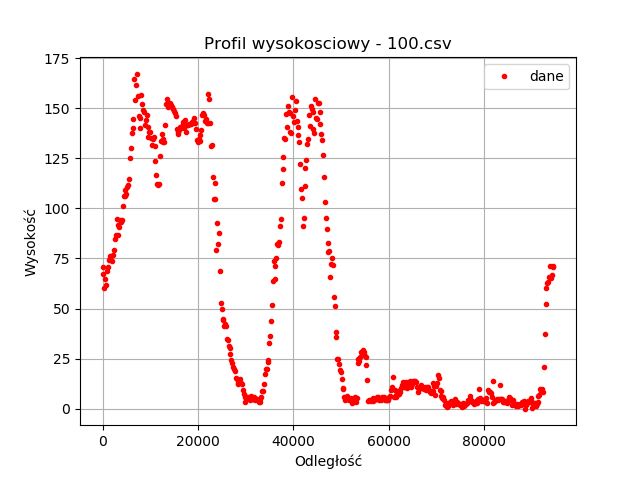
\includegraphics[width=\textwidth]{profile_wysokosciowe/100_pw.png}
        \caption{Profil wysokościowy trasy z pliku 100.csv}
    \end{minipage}
    \hfill
    \begin{minipage}[b]{0.4\textwidth}
        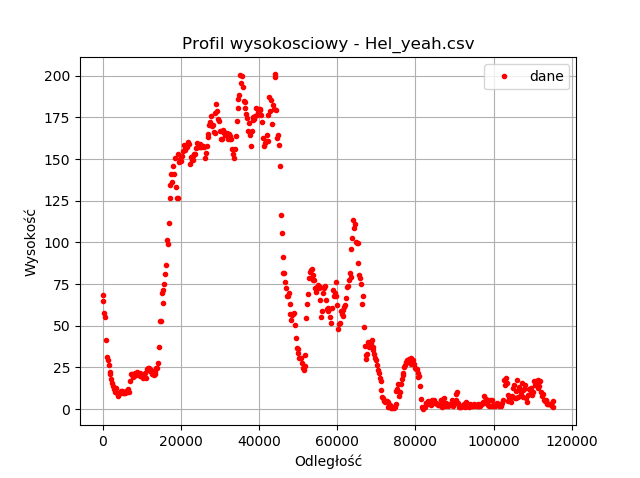
\includegraphics[width=\textwidth]{profile_wysokosciowe/hy_pw.png}
        \caption{Profil wysokościowy trasy z pliku helyeah.csv}
    \end{minipage}
    \centering
    \begin{minipage}[b]{0.4\textwidth}
        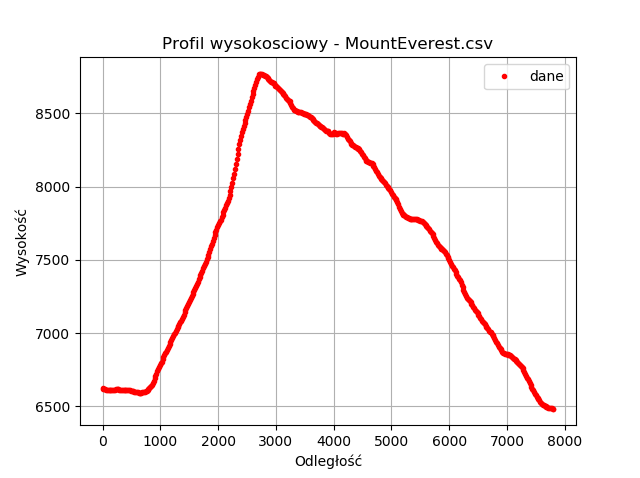
\includegraphics[width=\textwidth]{profile_wysokosciowe/me_pw.png}
        \caption{Profil wysokościowy trasy z pliku MountEverest.csv}
    \end{minipage}
    \hfill
    \begin{minipage}[b]{0.4\textwidth}
        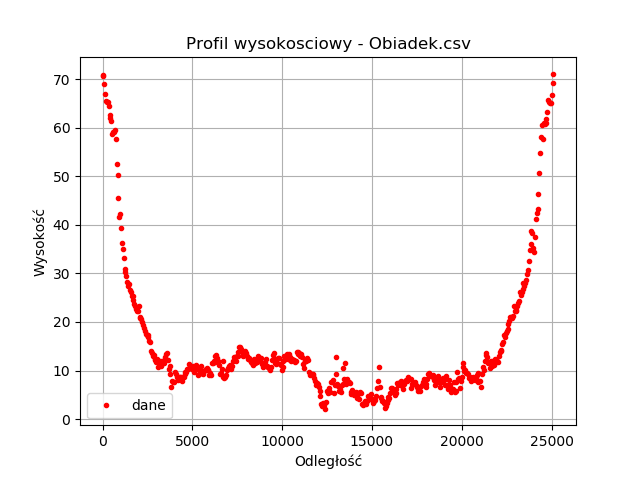
\includegraphics[width=\textwidth]{profile_wysokosciowe/ob_pw.png}
        \caption{Profil wysokościowy trasy z pliku Obiadek.csv}
    \end{minipage}
\end{figure}
\begin{figure}
    \begin{minipage}[b]{0.4\textwidth}
        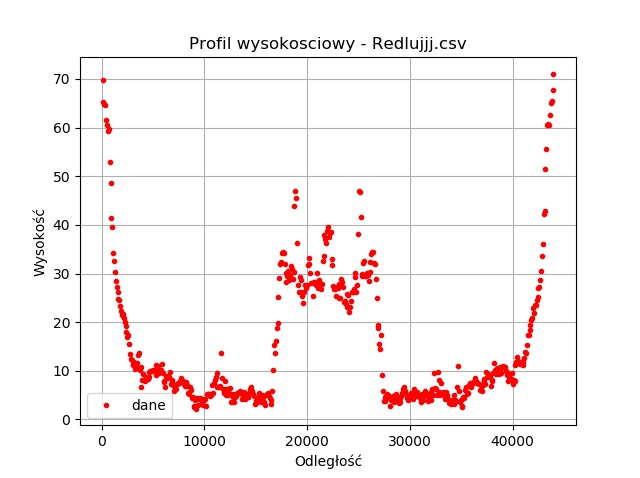
\includegraphics[width=\textwidth]{profile_wysokosciowe/red_pw.png}
        \caption{Profil wysokościowy trasy z pliku Redlujjj.csv}
    \end{minipage}
\end{figure}

\section{Interpolacja Langrange'a}
Interpolacja Lagrange'a jest interpolacją globalną, 
czyli przybliża wykres funkcji dla
wszystkich danych punktów jednocześnie. \\
W ogólności opiera się na wyznaczeniu zbioru funkcji,
 zwanego Bazą Lagrange'a. \\
 \begin{equation}
    \Phi_{i}(x) = \prod_{j=1, j \neq i}^{n} \frac{x-x_{j}}{x_{i} - x_{j}}
 \end{equation} \\
 Następnie, aby obliczyć funkcję interpolacyjną F(x) należy wykonać operację: \\
 \begin{equation} 
    F(x) = \sum_{i=1}^{n} y_{i} \Phi_{i}(x)
 \end{equation} \\
 Gdzie $P_{i} = (x_{i}, y_{i})$ oznacza punkt, 
 na podstawie którego jest przeprowadzana interpolacja.  
 \newpage
 \subsection{Metoda Lagrange'a a ilość punktów}
 Wraz ze wzrostem liczby punktów interpolacyjnych wzrasta dokładność funkcji interpolacyjnej.
 Warto jednak zauważyć, że na zewnętrznych wierzchołkach pojawiają się oscylacje. Jest to efekt Rungego,
 który jest największą wadą tej metody interpolacyjnej. Tak więc metoda nie jest skuteczna
 w swojej domyślnej postaci, ponieważ gdy jest zbyt mało punktów jest ona niedokładna,
 a gdy zbyt wiele to pojawia się efekt Rungego. Można ulepszyć tę metodę, generując przybliżenia przedziałami. \\
 Na poniższych wykresach przedstawiono efekty zastosowania metody interpolacyjnej Langrange'a.

\begin{figure}[h!]
    \centering
    \begin{minipage}[b]{0.4\textwidth}
        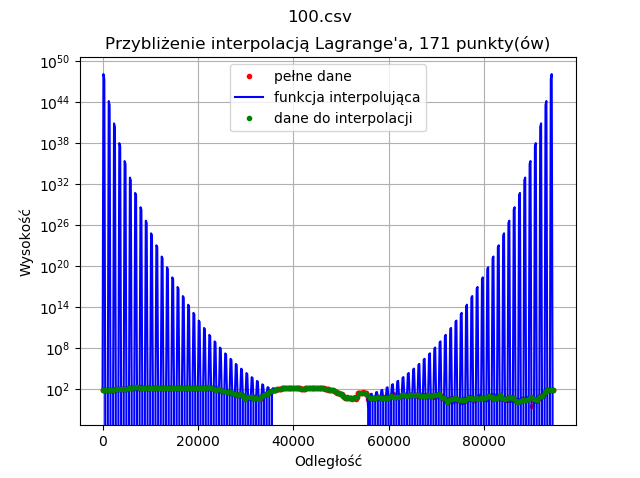
\includegraphics[width=\textwidth]{lagrange/rozna_dokladnosc/100_171punktow_cale.png}
        \caption{Wykres funkcji interpolowanej metodą Lagrange'a dla 171 punków.}
    \end{minipage}
    \hfill
    \begin{minipage}[b]{0.4\textwidth}
        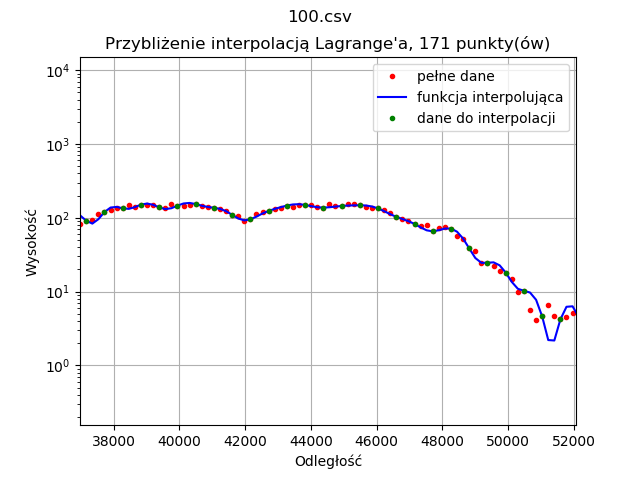
\includegraphics[width=\textwidth]{lagrange/rozna_dokladnosc/100_171_zb.png}
        \caption{Fragment przybliżenia funkcji interpolowanej metodą Lagrange'a dla 171 punktów}
    \end{minipage}
    \begin{minipage}[b]{0.4\textwidth}
        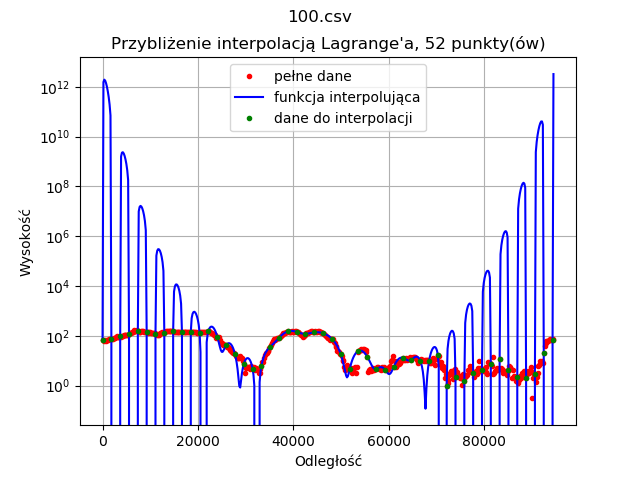
\includegraphics[width=\textwidth]{lagrange/rozna_dokladnosc/100_52_cale.png}
        \caption{Wykres funkcji interpolowanej metodą Lagrange'a dla 52 punków.}
    \end{minipage}
    \hfill
    \begin{minipage}[b]{0.4\textwidth}
        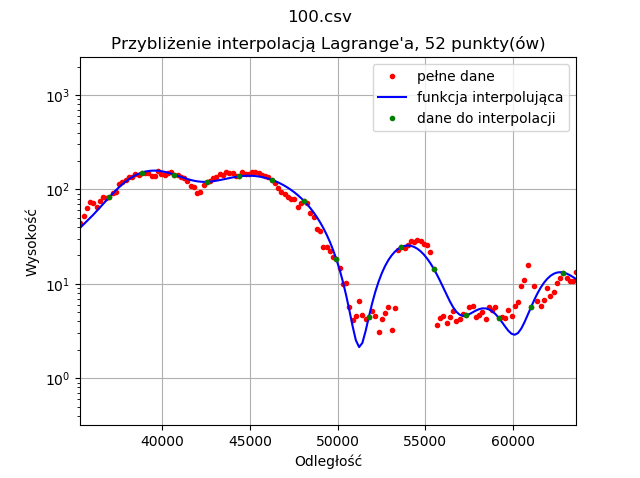
\includegraphics[width=\textwidth]{lagrange/rozna_dokladnosc/100_52_zb.png}
        \caption{Fragment wykresu funkcji interpolowanej metodą Lagrange'a dla 52 punków.}
    \end{minipage}
\end{figure}
\newpage
\subsection{Metoda interpolacji Lagrange'a a różne trasy}
Metoda interpolacji Lagrange'a jest skuteczna, gdy kolejne punkty układają się
w funkcję, której pierwsza pochodna nie zmienia często swojego znaku. Natomiast gdy 
interpolowana funkcja oscyluje wokół danej wartości, interpolacja metodą Lagrange'a
 jest mniej skuteczna. Na poniższych wykresach przedstawiono fragmenty interpolacji funkcji
 za pomocą metody Lagrange'a dla różnych tras:\\
\begin{figure}[h!]
    \center
    \begin{minipage}[b]{0.4\textwidth}
        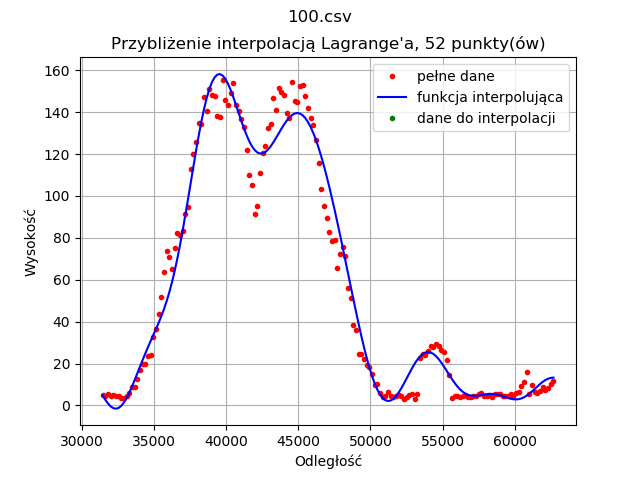
\includegraphics[width=\textwidth]{lagrange/rozne_trasy/100_52punkty_cale.png}
        \caption{Wykres interpolacji splajanami dla trasy 100.csv}
    \end{minipage}
    \hfill
    \begin{minipage}[b]{0.4\textwidth}
        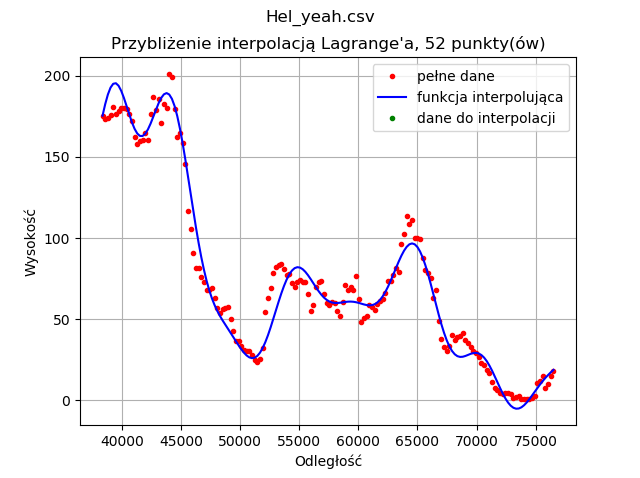
\includegraphics[width=\textwidth]{lagrange/rozne_trasy/hy_52punkty_cale.png}
        \caption{Fragment wykresu interpolacji splajanami dla trasy hellyeah.csv.}
    \end{minipage}
    \begin{minipage}[b]{0.4\textwidth}
        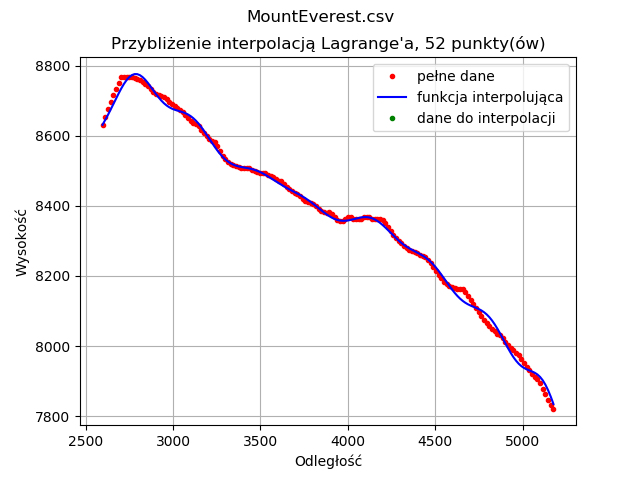
\includegraphics[width=\textwidth]{lagrange/rozne_trasy/me_52_cale.png}
        \caption{Wykres interpolacji splajanami dla trasy MountEverest.csv}
    \end{minipage}
    \hfill
    \begin{minipage}[b]{0.4\textwidth}
        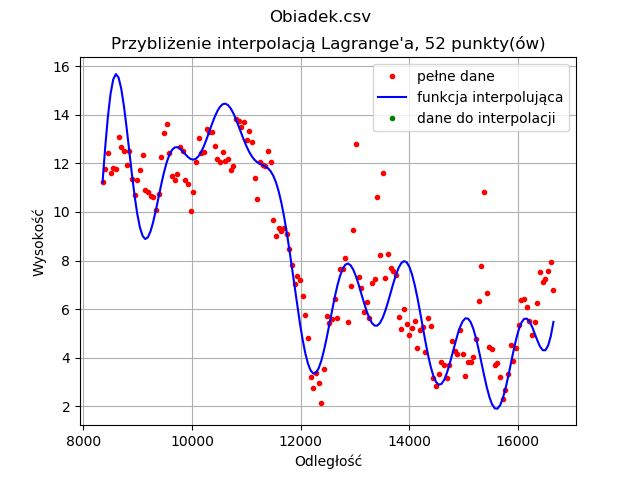
\includegraphics[width=\textwidth]{lagrange/rozne_trasy/obiadek_52_cale.png}
        \caption{Fragment wykresu interpolacji splajanami dla trasy Obiadek.csv}
    \end{minipage}
    \begin{minipage}[b]{0.4\textwidth}
        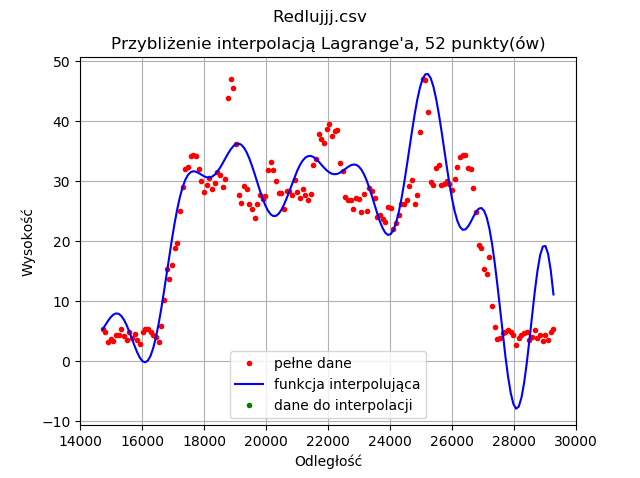
\includegraphics[width=\textwidth]{lagrange/rozne_trasy/red_52_cale.png}
        \caption{Fragment wykresu interpolacji splajanami dla trasy Redlujjj.csv}
    \end{minipage}
\end{figure}

\newpage
\section{Interpolacja splajnami}
Interpolacja splajnami polega na wyznaczaniu wielomianów n-tego stopnia na przedziałach pomiędzy
punktami wybranymi do interpolacji. W tym przypadku wyznaczane są wielomiany 3-ego stopnia.\\
Metoda polega na wyznaczeniu układu $4(n-1)$ równań, gdzie $n$ jest liczbą wybranych punktów.\\
Zakładamy, że pomiędzy punktami $x_{i}$ oraz $x_{i+1}$ istnieje wielomian $S_{i}(x) = a_{i}(x-x_{i})^3+b_{i}(x-x_{i})^2+c_{i}(x-x_{i})+d_{i}$. \\
Wtedy możemy wyznaczyć następujące równania: \\
\begin{itemize}
    \item{$S_{i}(x_{i}) = f(x_{i})$ - $(n-1)$ równań}
    \item{$S_{i}(x_{i+1}) = f(x_{i+1})$ - $(n-1)$ równań}
    \item{$S_{i}'(x_{i+1}) = S_{i+1}'(x_{i+1})$ - $(n-2)$ równania}
    \item{$S_{i}''(x_{i+1}) = S_{i+1}''(x_{i+1})$ - $(n-2)$ równania}
    \item {$S_{0}'(x_{0}) = S_{n-1}''(x_{n}) = 0$ - $(2)$ równania}
\end{itemize} 
Łącznie $4(n-1)$ równań. \\
Mamy $(n-1)$ przedziałów, więc musimy wyznaczyć $4(n-1)$ współczynników. \\
Powyższy układ równań możemy przedstawić w podstaci \textbf{Ax=b}. Rozwiązanie tego równania, 
po odpowiednim przestawieniu wierszy, jest przeprowadzane za pomocą faktoryzacji LU. 
W ten sposób wyznaczone jest $(n-1)$ wielomianów, pomiędzy $n$ punktami. 
\newpage
\subsection{Interpolacja splajnami a ilość punktów interpolacyjnych}
Wraz ze wzrostem liczby punktów wykorzystywanych do interpolacji rośnie dokładność 
przybliżenia, ale rosną też rozmiary macierzy oraz czas wykonywania obliczeń. Dla przykładu,
Na poniższych wykresach przedstawiono przybliżenia funkcji dla 256 i 52 punktów (dla pliku 100.csv): \\
\begin{figure}[h!]
    \center
    \begin{minipage}[b]{0.4\textwidth}
        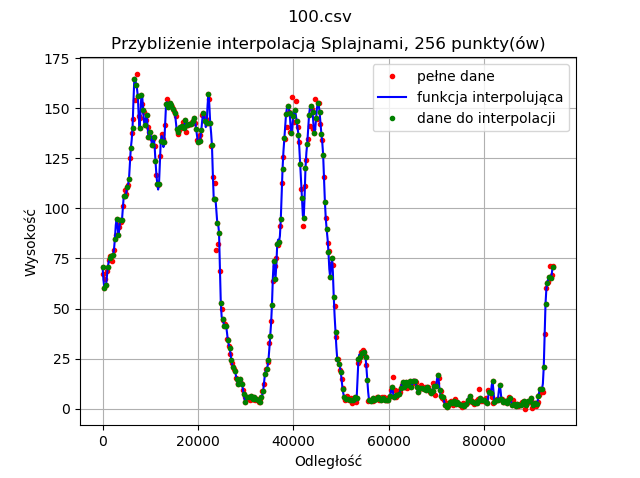
\includegraphics[width=\textwidth]{splajny/rozne_dokladnosci/100_256punktow_cale.png}
        \caption{Wykres interpolacji splajanami dla 256 punktów.}
    \end{minipage}
    \hfill
    \begin{minipage}[b]{0.4\textwidth}
        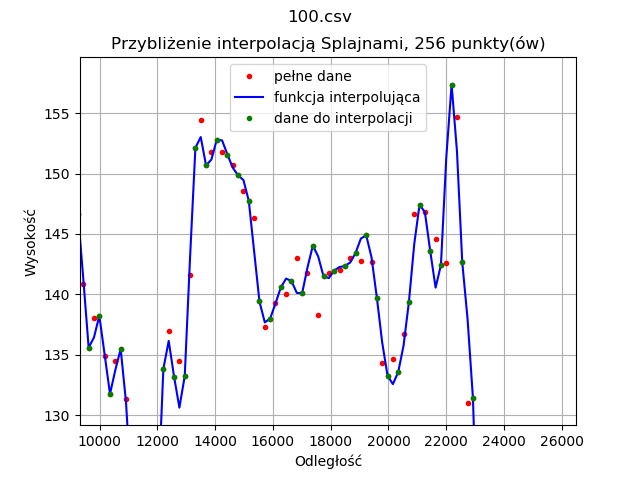
\includegraphics[width=\textwidth]{splajny/rozne_dokladnosci/100_256_zb.png}
        \caption{Fragment wykresu interpolacji splajanami dla 256 punktów.}
    \end{minipage}
    \begin{minipage}[b]{0.4\textwidth}
        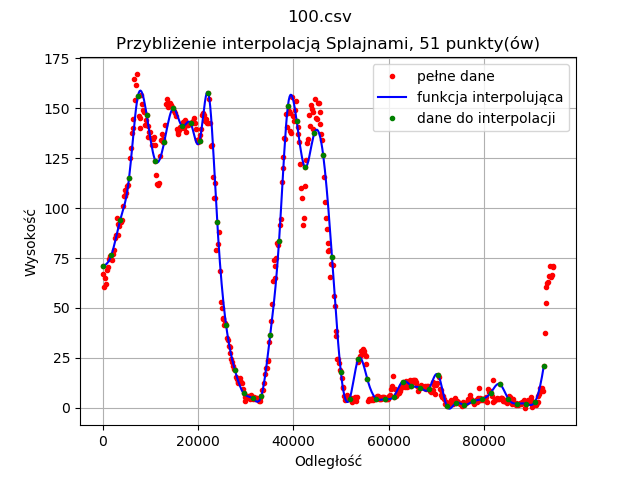
\includegraphics[width=\textwidth]{splajny/rozne_dokladnosci/100_52punkty_cale.png}
        \caption{Wykres interpolacji splajanami dla 52 punktów.}
    \end{minipage}
    \hfill
    \begin{minipage}[b]{0.4\textwidth}
        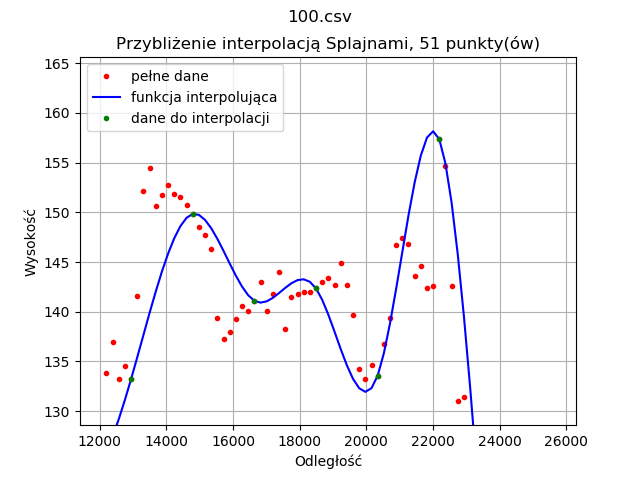
\includegraphics[width=\textwidth]{splajny/rozne_dokladnosci/100_52punkty_zblizenie.png}
        \caption{Fragment wykresu interpolacji splajanami dla 52 punktów.}
    \end{minipage}
\end{figure}

\newpage
\subsection{Interpolacja splajnami a różne typy danych}
Metoda interpolacji splajnami sprawdza się najlepiej, gdy interpolowana funkcja
przypomina funkcję wielomianową. Tak więc dla trasy Mount Everest, gdzie profil
początkowo gwałtownie rośnie, po czym gwałtownie maleje przybliżenie jest bardzo
dokładne na całym profilu. Natomiast w sytuacji, gdy wartości przybliżanej funkcji 
zmieniają się losowo, bądź pojawiają się "skoki", to funkcja interpolacyjna nie jest dokładna,
co można zaobserwować na wykresie trasy Redlujjj. Wykresy interpolacji dla różnych
rodzajó tras (wszystkie z wykorzystaniem 102 punktów) przedstawiono poniżej:
\begin{figure}[h!]
    \center
    \begin{minipage}[b]{0.4\textwidth}
        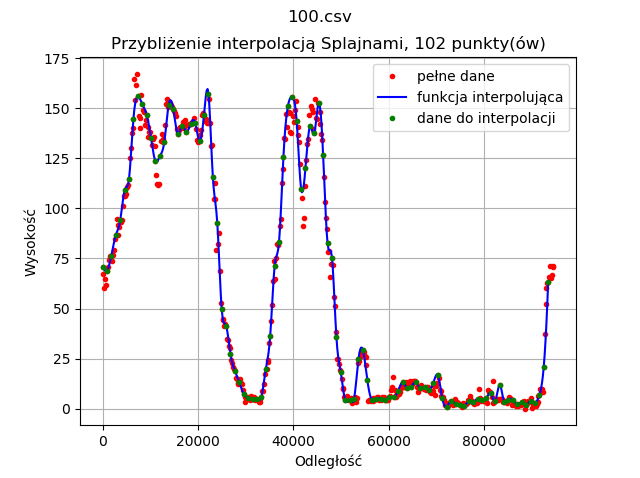
\includegraphics[width=\textwidth]{splajny/rozne_trasy/100_102.png}
        \caption{Wykres interpolacji splajanami dla trasy 100.csv}
    \end{minipage}
    \hfill
    \begin{minipage}[b]{0.4\textwidth}
        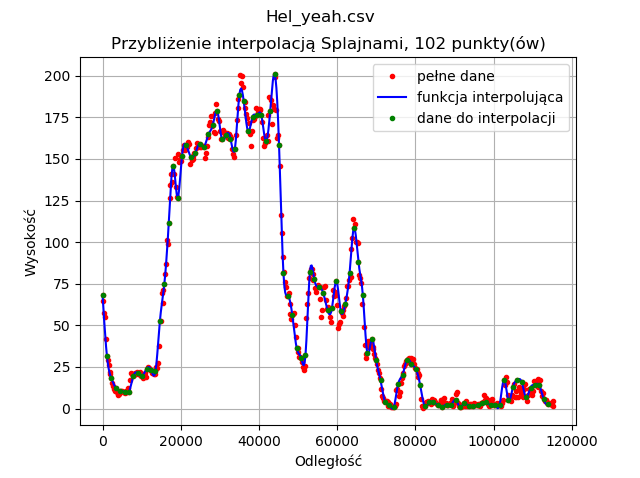
\includegraphics[width=\textwidth]{splajny/rozne_trasy/hy_102.png}
        \caption{Fragment wykresu interpolacji splajanami dla trasy hellyeah.csv.}
    \end{minipage}
    \begin{minipage}[b]{0.4\textwidth}
        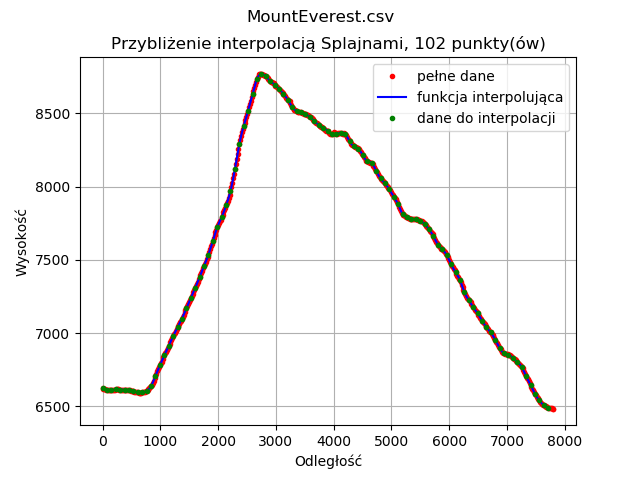
\includegraphics[width=\textwidth]{splajny/rozne_trasy/me_102.png}
        \caption{Wykres interpolacji splajanami dla trasy MountEverest.csv}
    \end{minipage}
    \hfill
    \begin{minipage}[b]{0.4\textwidth}
        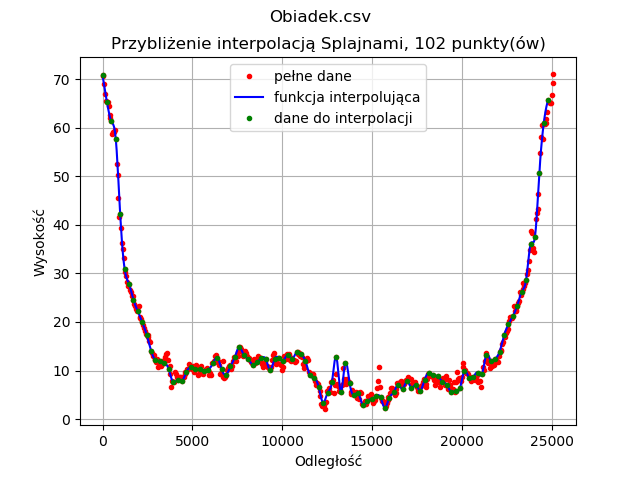
\includegraphics[width=\textwidth]{splajny/rozne_trasy/ob_102.png}
        \caption{Fragment wykresu interpolacji splajanami dla trasy Obiadek.csv}
    \end{minipage}
    \begin{minipage}[b]{0.4\textwidth}
        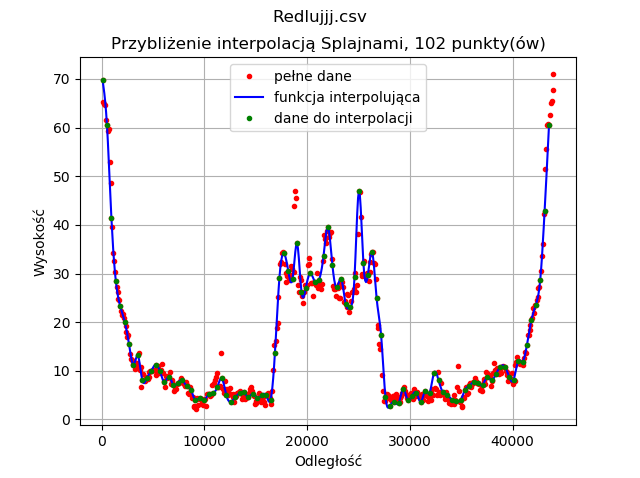
\includegraphics[width=\textwidth]{splajny/rozne_trasy/redl_102.png}
        \caption{Fragment wykresu interpolacji splajanami dla trasy Redlujjj.csv}
    \end{minipage}
\end{figure}

\section{Podsumowanie i wnioski}
Metoda interpolacji Lagrange'a wyznacza przybliżenia szybciej niż metoda 
interpolacji splajanami oraz ma mniejsze zapotrzebowanie pamięciowe. Jest jednak podatna 
na tzw. Efekt Rungego, czyli znaczące oscylacje w wierzchołkach zewnętrznych, przy dokłądnej
interpolacji wierzchołków wewnętrznych. Zbyt wiele punktów interpolacyjnych powoduje efekt Rungego, 
zbyt mała niedokładną interpolację. \\
Metoda interpolacji splajnami wymaga wyznaczenia układu równań oraz obliczenia go, przez co 
wymaga większych zasobów pamięciowych i czasowych. Nie jest jednak podatna na efekt Rungego. \\
Podsumowując, metoda interpolacji splajnami nadaje się lepiej do interpolacji profili 
wysokościowych niż metoda interpolacji Lagrange'a.
\end{document}